% Graphic for TeX using PGF
% Title: /home/ak/git/GM_Thesis/GM_Thesis_latex/GM_Thesis/img/Diagram1.dia
% Creator: Dia v0.97.3
% CreationDate: Mon May  2 16:26:03 2016
% For: ak
% \usepackage{tikz}
% The following commands are not supported in PSTricks at present
% We define them conditionally, so when they are implemented,
% this pgf file will use them.
\ifx\du\undefined
  \newlength{\du}
\fi
\setlength{\du}{15\unitlength}
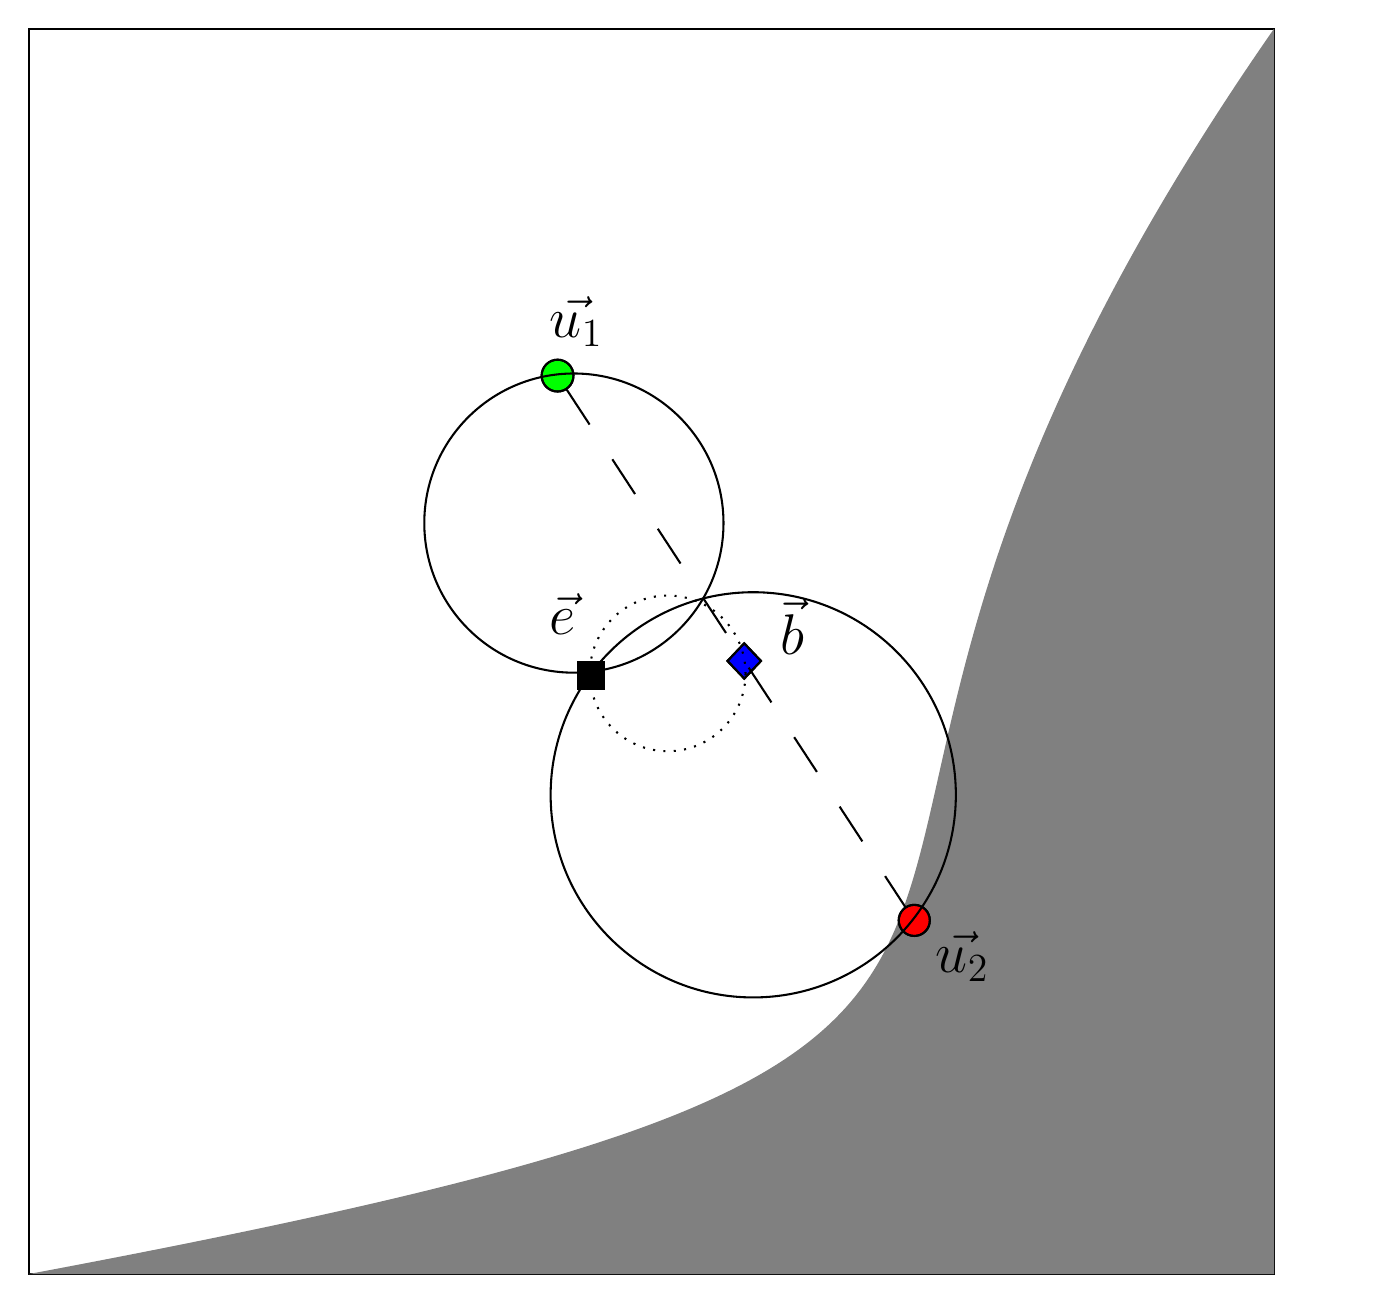
\begin{tikzpicture}
\pgftransformxscale{1.000000}
\pgftransformyscale{-1.000000}
\definecolor{dialinecolor}{rgb}{0.000000, 0.000000, 0.000000}
\pgfsetstrokecolor{dialinecolor}
\definecolor{dialinecolor}{rgb}{1.000000, 1.000000, 1.000000}
\pgfsetfillcolor{dialinecolor}
\pgfsetlinewidth{0.050000\du}
\pgfsetdash{}{0pt}
\pgfsetdash{}{0pt}
\pgfsetmiterjoin
\definecolor{dialinecolor}{rgb}{1.000000, 1.000000, 1.000000}
\pgfsetfillcolor{dialinecolor}
\fill (13.491964\du,2.844389\du)--(13.491964\du,32.844389\du)--(43.491964\du,32.844389\du)--(43.491964\du,2.844389\du)--cycle;
\definecolor{dialinecolor}{rgb}{0.000000, 0.000000, 0.000000}
\pgfsetstrokecolor{dialinecolor}
\draw (13.491964\du,2.844389\du)--(13.491964\du,32.844389\du)--(43.491964\du,32.844389\du)--(43.491964\du,2.844389\du)--cycle;
\pgfsetlinewidth{0.050000\du}
\pgfsetdash{}{0pt}
\pgfsetdash{}{0pt}
\pgfsetmiterjoin
\pgfsetbuttcap
{
\definecolor{dialinecolor}{rgb}{0.000000, 0.000000, 0.000000}
\pgfsetfillcolor{gray}
% was here!!!
\definecolor{dialinecolor}{rgb}{0.000000, 0.000000, 0.000000}
\pgfsetstrokecolor{dialinecolor}
\pgfpathmoveto{\pgfpoint{13.491964\du}{32.844389\du}}
\pgfpathcurveto{\pgfpoint{45.491964\du}{26.844389\du}}{\pgfpoint{27.491964\du}{25.844389\du}}{\pgfpoint{43.491964\du}{2.844389\du}}
\pgfpathlineto{\pgfpoint{43.491964\du}{32.844389\du}}
\pgfpathlineto{\pgfpoint{13.491964\du}{32.844389\du}}
\pgfusepath{fill}
}
\pgfsetlinewidth{0.050000\du}
\pgfsetdash{}{0pt}
\pgfsetdash{}{0pt}
\pgfsetbuttcap
\pgfsetmiterjoin
\pgfsetlinewidth{0.050000\du}
\pgfsetbuttcap
\pgfsetmiterjoin
\pgfsetdash{}{0pt}
\definecolor{dialinecolor}{rgb}{0.000000, 0.000000, 0.000000}
\pgfsetfillcolor{dialinecolor}
\fill (26.732258\du,18.100000\du)--(26.732258\du,18.745833\du)--(27.357258\du,18.745833\du)--(27.357258\du,18.100000\du)--cycle;
\definecolor{dialinecolor}{rgb}{0.000000, 0.000000, 0.000000}
\pgfsetstrokecolor{dialinecolor}
\draw (26.732258\du,18.100000\du)--(26.732258\du,18.745833\du)--(27.357258\du,18.745833\du)--(27.357258\du,18.100000\du)--cycle;
\pgfsetbuttcap
\pgfsetmiterjoin
\pgfsetdash{}{0pt}
\definecolor{dialinecolor}{rgb}{0.000000, 0.000000, 0.000000}
\pgfsetstrokecolor{dialinecolor}
\draw (26.732258\du,18.100000\du)--(26.732258\du,18.745833\du)--(27.357258\du,18.745833\du)--(27.357258\du,18.100000\du)--cycle;
\pgfsetlinewidth{0.050000\du}
\pgfsetdash{}{0pt}
\pgfsetdash{}{0pt}
\pgfsetbuttcap
\pgfsetmiterjoin
\pgfsetlinewidth{0.050000\du}
\pgfsetbuttcap
\pgfsetmiterjoin
\pgfsetdash{}{0pt}
\definecolor{dialinecolor}{rgb}{0.000000, 1.000000, 0.000000}
\pgfsetfillcolor{dialinecolor}
\pgfpathellipse{\pgfpoint{26.231719\du}{11.201094\du}}{\pgfpoint{0.383594\du}{0\du}}{\pgfpoint{0\du}{0.383594\du}}
\pgfusepath{fill}
\definecolor{dialinecolor}{rgb}{0.000000, 0.000000, 0.000000}
\pgfsetstrokecolor{dialinecolor}
\pgfpathellipse{\pgfpoint{26.231719\du}{11.201094\du}}{\pgfpoint{0.383594\du}{0\du}}{\pgfpoint{0\du}{0.383594\du}}
\pgfusepath{stroke}
\pgfsetbuttcap
\pgfsetmiterjoin
\pgfsetdash{}{0pt}
\definecolor{dialinecolor}{rgb}{0.000000, 0.000000, 0.000000}
\pgfsetstrokecolor{dialinecolor}
\pgfpathellipse{\pgfpoint{26.231719\du}{11.201094\du}}{\pgfpoint{0.383594\du}{0\du}}{\pgfpoint{0\du}{0.383594\du}}
\pgfusepath{stroke}
\pgfsetlinewidth{0.050000\du}
\pgfsetdash{}{0pt}
\pgfsetdash{}{0pt}
\definecolor{dialinecolor}{rgb}{0.000000, 0.000000, 0.000000}
\pgfsetstrokecolor{dialinecolor}
\pgfpathellipse{\pgfpoint{26.624998\du}{14.753711\du}}{\pgfpoint{3.603711\du}{0\du}}{\pgfpoint{0\du}{3.603711\du}}
\pgfusepath{stroke}
\pgfsetlinewidth{0.050000\du}
\pgfsetdash{}{0pt}
\pgfsetdash{}{0pt}
\pgfsetbuttcap
\pgfsetmiterjoin
\pgfsetlinewidth{0.050000\du}
\pgfsetbuttcap
\pgfsetmiterjoin
\pgfsetdash{}{0pt}
\definecolor{dialinecolor}{rgb}{0.000000, 0.000000, 1.000000}
\pgfsetfillcolor{dialinecolor}
\fill (30.728580\du,17.650000\du)--(31.132160\du,18.075205\du)--(30.728580\du,18.500411\du)--(30.325000\du,18.075205\du)--cycle;
\definecolor{dialinecolor}{rgb}{0.000000, 0.000000, 0.000000}
\pgfsetstrokecolor{dialinecolor}
\draw (30.728580\du,17.650000\du)--(31.132160\du,18.075205\du)--(30.728580\du,18.500411\du)--(30.325000\du,18.075205\du)--cycle;
\pgfsetbuttcap
\pgfsetmiterjoin
\pgfsetdash{}{0pt}
\definecolor{dialinecolor}{rgb}{0.000000, 0.000000, 0.000000}
\pgfsetstrokecolor{dialinecolor}
\draw (30.728580\du,17.650000\du)--(31.132160\du,18.075205\du)--(30.728580\du,18.500411\du)--(30.325000\du,18.075205\du)--cycle;
\pgfsetlinewidth{0.050000\du}
\pgfsetdash{{1.000000\du}{1.000000\du}}{0\du}
\pgfsetdash{{1.000000\du}{1.000000\du}}{0\du}
\pgfsetbuttcap
{
\definecolor{dialinecolor}{rgb}{0.000000, 0.000000, 0.000000}
\pgfsetfillcolor{dialinecolor}
% was here!!!
\definecolor{dialinecolor}{rgb}{0.000000, 0.000000, 0.000000}
\pgfsetstrokecolor{dialinecolor}
\draw (26.455689\du,11.543345\du)--(35.000000\du,24.600000\du);
}
\pgfsetlinewidth{0.050000\du}
\pgfsetdash{}{0pt}
\pgfsetdash{}{0pt}
\pgfsetbuttcap
\pgfsetmiterjoin
\pgfsetlinewidth{0.050000\du}
\pgfsetbuttcap
\pgfsetmiterjoin
\pgfsetdash{}{0pt}
\definecolor{dialinecolor}{rgb}{1.000000, 0.000000, 0.000000}
\pgfsetfillcolor{dialinecolor}
\pgfpathellipse{\pgfpoint{34.825000\du}{24.325000\du}}{\pgfpoint{0.375000\du}{0\du}}{\pgfpoint{0\du}{0.375000\du}}
\pgfusepath{fill}
\definecolor{dialinecolor}{rgb}{0.000000, 0.000000, 0.000000}
\pgfsetstrokecolor{dialinecolor}
\pgfpathellipse{\pgfpoint{34.825000\du}{24.325000\du}}{\pgfpoint{0.375000\du}{0\du}}{\pgfpoint{0\du}{0.375000\du}}
\pgfusepath{stroke}
\pgfsetbuttcap
\pgfsetmiterjoin
\pgfsetdash{}{0pt}
\definecolor{dialinecolor}{rgb}{0.000000, 0.000000, 0.000000}
\pgfsetstrokecolor{dialinecolor}
\pgfpathellipse{\pgfpoint{34.825000\du}{24.325000\du}}{\pgfpoint{0.375000\du}{0\du}}{\pgfpoint{0\du}{0.375000\du}}
\pgfusepath{stroke}
\pgfsetlinewidth{0.050000\du}
\pgfsetdash{}{0pt}
\pgfsetdash{}{0pt}
\definecolor{dialinecolor}{rgb}{0.000000, 0.000000, 0.000000}
\pgfsetstrokecolor{dialinecolor}
\pgfpathellipse{\pgfpoint{30.945619\du}{21.299999\du}}{\pgfpoint{4.880840\du}{0\du}}{\pgfpoint{0\du}{4.880840\du}}
\pgfusepath{stroke}
\pgfsetlinewidth{0.050000\du}
\pgfsetdash{{\pgflinewidth}{0.200000\du}}{0cm}
\pgfsetdash{{\pgflinewidth}{0.200000\du}}{0cm}
\definecolor{dialinecolor}{rgb}{0.000000, 0.000000, 0.000000}
\pgfsetstrokecolor{dialinecolor}
\pgfpathellipse{\pgfpoint{28.885285\du}{18.374589\du}}{\pgfpoint{1.875000\du}{0\du}}{\pgfpoint{0\du}{1.875000\du}}
\pgfusepath{stroke}
% setfont left to latex
\definecolor{dialinecolor}{rgb}{0.000000, 0.000000, 0.000000}
\pgfsetstrokecolor{dialinecolor}
\node[anchor=west] at (27.697785\du,18.974590\du){};
% setfont left to latex
\definecolor{dialinecolor}{rgb}{0.000000, 0.000000, 0.000000}
\pgfsetstrokecolor{dialinecolor}
\node[anchor=west] at (25.797785\du,16.949589\du){\huge$\vec{e}$};
% setfont left to latex
\definecolor{dialinecolor}{rgb}{0.000000, 0.000000, 0.000000}
\pgfsetstrokecolor{dialinecolor}
\node[anchor=west] at (25.797785\du,9.899589\du){\huge$\vec{u_1}$};
% setfont left to latex
\definecolor{dialinecolor}{rgb}{0.000000, 0.000000, 0.000000}
\pgfsetstrokecolor{dialinecolor}
\node[anchor=west] at (31.347785\du,17.249589\du){\huge$\vec{b}$};
% setfont left to latex
\definecolor{dialinecolor}{rgb}{0.000000, 0.000000, 0.000000}
\pgfsetstrokecolor{dialinecolor}
\node[anchor=west] at (35.097785\du,25.199589\du){\huge$\vec{u_2}$};
\end{tikzpicture}
